\section{Разбиение группы в смежные классы}

\begin{shdef}
    \begin{definition} [Разбиение группы на смежные классы]
    \leavevmode \nl

    Пусть \( G \) — группа, а \( H \) — её подгруппа. Для любого элемента \( a \in G \) \textbf{левый смежный класс} подгруппы \( H \) по элементу \( a \) определяется как множество:
    \[
    aH = \{ a \circ h \mid h \in H \}.
    \]
    Аналогично, \textbf{правый смежный класс} подгруппы \( H \) по элементу \( a \) определяется как множество:
    \[
    Ha = \{ h \circ a \mid h \in H \}.
    \]

    Множество всех левых (или правых) смежных классов подгруппы \( H \) в группе \( G \) называется \textbf{разбиением группы \( G \) на смежные классы по подгруппе \( H \)}.
    \end{definition}
\end{shdef}

\begin{shex}
    \textbf{Свойства смежных классов:} (определим для левых смежных классов, для \\правых аналогично)
    \begin{enumerate}
        \item \( \forall a \in H \quad aH = H \)
        \item \( a \in aH \quad \forall a \in G \)
        \item \( aH = bH \iff b^{-1} \circ a \in H \)
        \item Любые два левых смежных класса \( aH \) и \( bH \) либо совпадают, либо не пересекаются
    \end{enumerate}
\end{shex}

\begin{proof}
    \leavevmode \nl 
    
    \begin{enumerate}
    \item Пусть \( a \in H \). Тогда:
    \[
    aH = \{ a \circ h \mid h \in H \}.
    \]
    
    Поскольку \( H \) — подгруппа, для любого \( h \in H \) элемент \( a \circ h \) также принадлежит \( H \). Следовательно, \( aH \subseteq H \). \\
    
    Обратно, для любого \( h \in H \) элемент \( h = a \circ (a^{-1} \circ h) \), где \( a^{-1} \circ h \in H \) (так как \( H \) — подгруппа). Таким образом, \( H \subseteq aH \). \\
    

    \item Поскольку \( e \in H \) (нейтральный элемент), то:
    \[
    a = a \circ e \in aH.
    \]

    \item 
    \boxed{\Rightarrow} Пусть \( aH = bH \). Тогда существуют \( h_1, h_2 \in H \) такие, что:
    \[
    a \circ h_1 = b \circ h_2.
    \]
    "Умножаем" \; обе части равенства слева на \( b^{-1} \):
    \[
    b^{-1} \circ a \circ h_1 = h_2.
    \]
    Теперь "домножаем" \; обе части на \( h_1^{-1} \):
    \[
    b^{-1} \circ a = h_2 \circ h_1^{-1}.
    \]
    Поскольку \( H \) — подгруппа, \( h_2 \circ h_1^{-1} \in H \). Следовательно, \( b^{-1} \circ a \in H \).

    
    \boxed{\Leftarrow} Пусть \( b^{-1} \circ a \in H \). Тогда:
    \[
    b^{-1} \circ aH = H \quad \text{(по свойству 1)}.
    \]
    "Умножаем" \; обе части равенства слева на \( b \):
    \[
    aH = b \circ (b^{-1} \circ aH) = bH.
    \]
    Таким образом, \( aH = bH \).

    \item Пусть \( aH \) и \( bH \) — два левых смежных класса. Если \( aH \; \cap \; bH \neq \emptyset \), то \(\exists x \in aH \cap bH \). Тогда:
    \[
    x = a \circ h_1 = b \circ h_2 \quad \text{для некоторых } h_1, h_2 \in H.
    \]
    Отсюда:
    \[
    b^{-1} \circ a = h_2 \circ h_1^{-1} \in H.
    \]
    По свойству 3, это означает, что \( aH = bH \). Следовательно, если \( aH \) и \( bH \) пересекаются, то они совпадают.
    \end{enumerate}
\end{proof}

\textbf{Пример смежных классов:}
\begin{enumerate}

    \item Пусть \( G = \mathbb{R}^2 \) — группа векторов на плоскости с операцией сложения, \\
    \( H \) — подгруппа, состоящая из всех векторов, лежащих на прямой \( y = x \):
    \[
    H = \{ (x, x) \mid x \in \mathbb{R} \}.
    \]
    Тогда левые (и правые) смежные классы \( a + H \) — это параллельные прямые, смещённые на вектор \( a \).

    
    \item Пусть \( G = \mathbb{C} \setminus \{ 0 \} \) — группа ненулевых комплексных чисел с операцией \\умножения,
    \( H \) — подгруппа, состоящая из всех комплексных чисел, лежащих на единичной окружности:
    \[
    H = \{ z \in \mathbb{C} \mid |z| = 1 \}.
    \]
    Тогда левые (и правые) смежные классы \( z_{0}H \) — это окружности с центром в нуле и радиусом \( |z_{0}| \).

\end{enumerate}

\begin{center}
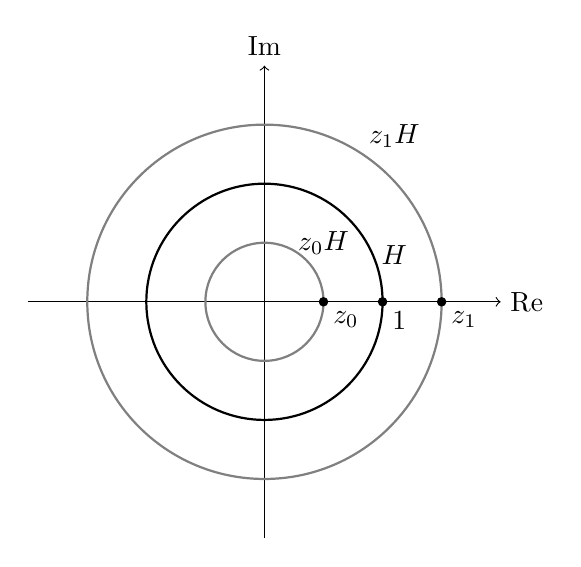
\begin{tikzpicture}[scale=1.5]

    % Оси
    \draw[->] (-2, 0) -- (2, 0) node[right] {Re};
    \draw[->] (0, -2) -- (0, 2) node[above] {Im};

    
    \draw[thick, black] (0, 0) circle (1);
    \node at (1.1, 0.4) {\( H \)}; 

    
    \draw[thick, gray] (0, 0) circle (0.5);
    \node at (0.5, 0.5) {\( z_0H \)}; 

    \draw[thick, gray] (0, 0) circle (1.5);
    \node at (1.1, 1.4) {\( z_1H \)}; 

    % Точки
    \filldraw (1, 0) circle (1pt) node[below right] {\( 1 \)};
    \filldraw (0.5, 0) circle (1pt) node[below right] {\( z_0 \)};
    \filldraw (1.5, 0) circle (1pt) node[below right] {\( z_1 \)};

\end{tikzpicture}
\end{center}


\begin{shth}
    \begin{theorem}
        Пусть \( G \) — конечная группа порядка \( n \), \( H \) — подгруппа порядка \( k \). Пусть \( j \) — количество смежных классов группы \( G \) по подгруппе \( H \). Тогда 
        \[
        n = k \cdot j.
        \]
    \end{theorem}
\end{shth}

\begin{proof}
    Пусть \( h_1, h_2 \in H \), \( g \in G \) — произвольный элемент группы \( G \). Рассмотрим отображение:
    \[
    \phi: H \to gH, \quad \phi(h) = g \circ h.
    \]
    Покажем, что \( \phi \) является биекцией.

    \begin{enumerate}
        \item Инъективность:
            Пусть \( \phi(h_1) = \phi(h_2) \). Тогда:
            \[
            g \circ h_1 = g \circ h_2.
            \]
            Умножим обе части равенства слева на \( g^{-1} \):
            \[
            g^{-1} \circ (g \circ h_1) = g^{-1} \circ (g \circ h_2) \implies (g^{-1} \circ g) \circ h_1 = (g^{-1} \circ g) \circ h_2.
            \]
            Так как \( g^{-1} \circ g = e \), то:
            \[
            e \circ h_1 = e \circ h_2 \implies h_1 = h_2.
            \]
            Таким образом, \( \phi \) инъективно.

        \item Сюръективность:
            Для любого элемента \( y \in gH \) существует \( h \in H \), такой что \( y = g \circ h \). По определению \( \phi \), это означает, что \( \phi(h) = y \). Следовательно, \( \phi \) сюръективно.
    \end{enumerate}

    Так как \( \phi \) биективно, то \( |gH| = |H| = k \). Аналогично, все смежные классы \( gH \) имеют одинаковое количество элементов \( k \).

    Поскольку группа \( G \) разбивается на \( j \) смежных классов, каждый из которых \\содержит \( k \) элементов, то общее количество элементов в группе \( G \) равно:
    \[
    n = k \cdot j.
    \]
\end{proof}


\begin{shcor}
    \begin{corollary}\boxed{\textbf{Теорема Лагранжа}}.
    \leavevmode \nl 
    
        Пусть \( G \) — конечная группа. Тогда порядок любой подгруппы \( H \subseteq G \) является делителем порядка группы \( G \). То есть, если \( |G| = n \) и \( |H| = k \), то \( k \) делит \( n \).
    \end{corollary}
\end{shcor}


\begin{shcor}
    \begin{corollary}
    \leavevmode \nl 

        Если группа \( G \) конечна, то порядок любого элемента \( g \in G \) является делителем порядка группы \( G \).
    \end{corollary}
\end{shcor}

\begin{shcor}
    \begin{corollary}
        Если порядок конечной группы \( G \) является простым числом, то \( G \) является циклической группой.
    \end{corollary}
\end{shcor}

\begin{proof}
    Пусть \( |G| = p \), где \( p \) — простое число. Рассмотрим произвольный элемент \( g \in G \), отличный от нейтрального элемента \( e \). 

    По следствию из теоремы Лагранжа, порядок элемента \( g \) делит порядок группы \( G \). Так как \( p \) — простое число, то возможны только два случая:
    \begin{enumerate}
        \item Порядок элемента \( g \) равен \( 1 \). Но это возможно только если \( g = e \), что противоречит выбору \( g \).
        \item Порядок элемента \( g \) равен \( p \).
    \end{enumerate}

    Таким образом, порядок элемента \( g \) равен \( p \), и циклическая подгруппа \( \langle g \rangle \), порождённая элементом \( g \), содержит \( p \) элементов. Следовательно, \( \langle g \rangle = G \), и группа \( G \) является циклической.
\end{proof}

\begin{shdef}
    \begin{definition}[Нормальный делитель]
    \leavevmode \nl 
    
        Подгруппа \( H \) группы \( G \) называется \textbf{нормальным делителем}, если \( \forall a \in G \) левые и правые смежные классы группы \( G \) по подгруппе \( H \) совпадают, то есть:
        \[
        aH = Ha.
        \]
        Обозначение: \( H \triangleleft G \).
    \end{definition}
\end{shdef}


\begin{remark}
    Если группа \( G \) абелева, то \textbf{любая её подгруппа \( H \)} является нормальным делителем. Это следует из того, что в абелевой группе левые и правые смежные классы всегда совпадают:
    \[
    aH = \{ a \circ h \mid h \in H \} = \{ h \circ a \mid h \in H \} = Ha.
    \]
\end{remark}

\begin{shth}
    \begin{theorem}
        Пусть \( H \triangleleft G \) — нормальный делитель группы \( G \), и \( \circ \) — групповая операция. Тогда композиция смежных классов \( (aH) \) и \( (bH) \) определяется формулой:
        \[
        (aH) \circ (bH) = (a \circ b)H.
        \]
    \end{theorem}
\end{shth}

\begin{proof}
    Рассмотрим композицию смежных классов \( (aH) \) и \( (bH) \). \\Поскольку \( H \) — нормальный делитель, выполняется \( Hb = bH \). Тогда:
    \[
    (aH) \circ (bH) = a(Hb)H = a(bH)H = (a \circ b)(HH).
    \]
    Так как \( H \) — подгруппа, то \( HH = H \). Следовательно:
    \[
    (a \circ b)(HH) = (a \circ b)H.
    \]
    Таким образом, \( (aH) \circ (bH) = (a \circ b)H \).
\end{proof}

\clearpage
\section{Гомоморфизм. Фактор-Группы}

\begin{shdef}
    \begin{definition}[Гомоморфизм]
        Пусть \( (G, \circ) \) — группа, а \( (X, \star) \) — множество \( X \) с бинарной операцией \( \star \). Отображение \( \phi: G \to X \) называется \textbf{гомоморфизмом}, если для любых элементов \( a, b \in G \) выполняется:
        \[
        \phi(a \circ b) = \phi(a) \star \phi(b).
        \]
        

        \begin{remark}
            Гомоморфизм — это более общее понятие, чем изоморфизм. В отличие от \\изоморфизма, гомоморфизм не требует биективности, но всегда сохраняет \\алгебраическую структуру. Гомоморфизм может быть:
            \begin{itemize}
                \item \textbf{Инъективным}, если разные элементы \( G \) переходят в разные элементы \( X \).
                \item \textbf{Сюръективным}, если образ \( \phi(G) \) совпадает с \( X \).
                \item \textbf{Биективным} (изоморфизм), если он одновременно инъективен и сюръективен.
            \end{itemize}
        \end{remark}
    \end{definition}
\end{shdef}

\begin{shdef}
    \begin{definition}[Эндоморфизм]
        Пусть \( (G, \circ) \) — группа. 
        
        Отображение \( \phi: G \to G \) называется \textbf{эндоморфизмом}, если:
        \begin{enumerate}
            \item \( \phi \) является гомоморфизмом, то есть \(\forall a, b \in G \) выполняется:
                  \[
                  \phi(a \circ b) = \phi(a) \circ \phi(b);
                  \]
            \item \( \phi \) отображает группу \( G \) в себя, то есть \( \phi(G) \subseteq G \).
        \end{enumerate}
    \end{definition}
\end{shdef}

\begin{shth}
    \begin{theorem}
        Пусть \( G \) — группа, а \( X \) — множество с бинарной операцией \( \star \). Если \( \phi: G \to X \) — гомоморфизм, то \( X \) является группой относительно операции \( \star \).
    \end{theorem}
\end{shth}

\begin{proof}
    Чтобы доказать, что \( X \) — группа, проверим выполнение аксиом группы:
    \begin{enumerate}
        \item Ассоциативность:
              Для любых \( x, y, z \in X \) существуют \( a, b, c \in G \), такие что \( x = \phi(a) \), \( y = \phi(b) \), \( z = \phi(c) \). Тогда:
              \[
              (x \star y) \star z = (\phi(a) \star \phi(b)) \star \phi(c) = \phi(a \circ b) \star \phi(c) = \phi((a \circ b) \circ c).
              \]
              Аналогично:
              \[
              x \star (y \star z) = \phi(a) \star (\phi(b) \star \phi(c)) = \phi(a) \star \phi(b \circ c) = \phi(a \circ (b \circ c)).
              \]
              Поскольку \( G \) — группа, \( (a \circ b) \circ c = a \circ (b \circ c) \), следовательно:
              \[
              (x \star y) \star z = x \star (y \star z).
              \]

        \item Нейтральный элемент:
              Пусть \( e_G \) — нейтральный элемент группы \( G \). \\Положим \( e_X = \phi(e_G) \). Тогда для любого \( x \in X \), где \( x = \phi(a) \), выполняется:
              \[
              e_X \star x = \phi(e_G) \star \phi(a) = \phi(e_G \circ a) = \phi(a) = x.
              \]
              Аналогично:
              \[
              x \star e_X = \phi(a) \star \phi(e_G) = \phi(a \circ e_G) = \phi(a) = x.
              \]
              Таким образом, \( e_X \) — нейтральный элемент в \( X \).

        \item Обратный элемент:
              Для любого \( x \in X \), где \( x = \phi(a) \), рассмотрим элемент \( y = \phi(a^{-1}) \), где \( a^{-1} \) — обратный к \( a \) в \( G \). Тогда:
              \[
              x \star y = \phi(a) \star \phi(a^{-1}) = \phi(a \circ a^{-1}) = \phi(e_G) = e_X.
              \]
              Аналогично:
              \[
              y \star x = \phi(a^{-1}) \star \phi(a) = \phi(a^{-1} \circ a) = \phi(e_G) = e_X.
              \]
              Таким образом, \( y \) — обратный элемент к \( x \) в \( X \).
    \end{enumerate}

    Все аксиомы группы выполнены, следовательно, \( X \) — группа.
\end{proof}

\vspace{0.3cm}

\begin{shdef}
    \begin{definition}[Ядро гомоморфизма]
    \leavevmode \nl 
    
        Пусть \( \phi: G \to X \) — гомоморфизм. \textbf{Ядром} гомоморфизма \( \phi \) называется множество всех элементов группы \( G \), которые отображаются в нейтральный элемент \( e_X \) группы \( X \). Формально:
        \[
        \ker(\phi) = \{ g \in G \mid \phi(g) = e_X \}.
        \]
    \end{definition}
\end{shdef}

\begin{shth}
    \begin{theorem}
        Пусть \( \phi: G \to X \) — гомоморфизм группы \( (G, \circ) \) в группу \( X \) с групповой операцией \( \star \). Тогда ядро \( \ker(\phi) \) является:
        \begin{enumerate}
            \item Подгруппой группы \( G \).
            \item Нормальным делителем группы \( G \).
        \end{enumerate}
    \end{theorem}
\end{shth}


\begin{proof}
    Докажем оба утверждения.

    \begin{enumerate}
        \item Ядро \( \ker(\phi) \) — подгруппа группы \( G \):
              Проверим выполнение аксиом подгруппы:
              \begin{itemize}
                  \item Замыкание:
                        Пусть \( a, b \in \ker(\phi) \). Тогда:
                        \[
                        \phi(a \circ b) = \phi(a) \star \phi(b) = e_X \star e_X = e_X.
                        \]
                        Следовательно, \( a \circ b \in \ker(\phi) \).

                  \item Нейтральный элемент:
                        Поскольку \( \phi(e_G) = e_X \), то \( e_G \in \ker(\phi) \).

                  \item Обратный элемент:
                        Пусть \( a \in \ker(\phi) \). Тогда:
                        \[
                        \phi(a^{-1}) = (\phi(a))^{-1} = e_X^{-1} = e_X.
                        \]
                        Следовательно, \( a^{-1} \in \ker(\phi) \).
              \end{itemize}
              Таким образом, \( \ker(\phi) \) — подгруппа группы \( G \).

        \item Ядро \( \ker(\phi) \) — нормальный делитель группы \( G \):
              Покажем, что для любого \( a \in G \) выполняется \( a^{-1} \ker(\phi) a \subseteq \ker(\phi) \).

              Рассмотрим произвольный элемент \( h \in \ker(\phi) \) и произвольный элемент \( a \in G \). Покажем, что \( a^{-1} \circ h \circ a \in \ker(\phi) \). Применим гомоморфизм \( \phi \) к этому элементу:
              \[
              \phi(a^{-1} \circ h \circ a) = \phi(a^{-1}) \star \phi(h) \star \phi(a).
              \]
              Поскольку \( h \in \ker(\phi) \), то \( \phi(h) = e_X \). Также, так как \( \phi \) — гомоморфизм, выполняется \( \phi(a^{-1}) = (\phi(a))^{-1} \). Подставляем:
              \[
              \phi(a^{-1} \circ h \circ a) = (\phi(a))^{-1} \star e_X \star \phi(a) = (\phi(a))^{-1} \star \phi(a) = e_X.
              \]
              Таким образом, \( \phi(a^{-1} \circ h \circ a) = e_X \), что означает \( a^{-1} \circ h \circ a \in \ker(\phi) \).

              Мы показали, что для любого \( a \in G \) и любого \( h \in \ker(\phi) \) выполняется \( a^{-1} \circ h \circ a \in \ker(\phi) \). Это означает, что:
              \[
              a^{-1} \ker(\phi) a \subseteq \ker(\phi).
              \]

              Теперь "домножим" обе части включения справа на \( a \). Получим:
              \[
              \ker(\phi) a \subseteq \ker(\phi) a.
              \]
              

              Теперь покажем обратное включение. Рассмотрим произвольный элемент \( h \in \ker(\phi) \) и произвольный элемент \( a \in G \). Покажем, что \( a \circ h \circ a^{-1} \in \ker(\phi) \). Применим гомоморфизм \( \phi \) к этому элементу:
              \[
              \phi(a \circ h \circ a^{-1}) = \phi(a) \star \phi(h) \star \phi(a^{-1}).
              \]
              Поскольку \( h \in \ker(\phi) \), то \( \phi(h) = e_X \). Также, так как \( \phi \) — гомоморфизм, выполняется \( \phi(a^{-1}) = (\phi(a))^{-1} \). Подставляем:
              \[
              \phi(a \circ h \circ a^{-1}) = \phi(a) \star e_X \star (\phi(a))^{-1} = \phi(a) \star (\phi(a))^{-1} = e_X.
              \]
              Таким образом, \( \phi(a \circ h \circ a^{-1}) = e_X \), что означает \( a \circ h \circ a^{-1} \in \ker(\phi) \).

              Мы показали, что для любого \( a \in G \) и любого \( h \in \ker(\phi) \) выполняется \( a \circ h \circ a^{-1} \in \ker(\phi) \). Это означает, что:
              \[
              a \ker(\phi) a^{-1} \subseteq \ker(\phi).
              \]

              Таким образом, мы получили два включения:
              \[
              a^{-1} \ker(\phi) a \subseteq \ker(\phi) \quad \text{и} \quad a \ker(\phi) a^{-1} \subseteq \ker(\phi).
              \]
              
              Из этих включений следует, что:
              \[
              a \ker(\phi) = \ker(\phi) a.
              \]
              Это и есть определение нормального делителя.
    \end{enumerate}
\end{proof}

\clearpage

\begin{shdef}
    \begin{definition}[Фактор-группа]
    \leavevmode \nl 
    
        Пусть \( G \) — группа, а \( H \triangleleft G \) — её нормальный делитель. \textbf{Фактор-группой} группы \( G \) по подгруппе \( H \) называется множество всех смежных классов \( G \) по \( H \) с операцией, определённой следующим образом:
        \[
        (aH) \circ (bH) = (a \circ b)H,
        \]
        где \( a, b \in G \), а \( \circ \) — групповая операция в \( G \). Обозначение: \( G / H \).
    \end{definition}
\end{shdef}

\begin{shth}
    \begin{theorem}
        Пусть \( G \) — циклическая группа, порождённая элементом \( g \). Тогда:
        \begin{enumerate}
            \item Если \( G \) бесконечна, то \( G \cong \mathbb{Z} \) (группа целых чисел с операцией сложения).
            \item Если \( G \) конечна порядка \( n \), то \( G \cong \mathbb{Z}_n \) (группа целых чисел по модулю \( n \) с операцией сложения).
        \end{enumerate}
    \end{theorem}
\end{shth}

\begin{proof}
    Докажем оба утверждения.

    \begin{enumerate}
        \item Случай бесконечной циклической группы:
              Пусть \( G = \langle g \rangle \) — бесконечная циклическая группа. Поскольку \( G \) бесконечна, \( \forall k_1, k_2 \in \mathbb{Z} \), если \( k_1 \neq k_2 \), то \( g^{k_1} \neq g^{k_2} \). Построим отображение \( \phi: G \to \mathbb{Z} \) по правилу:
              \[
              \phi(g^k) = k.
              \]
              Покажем, что \( \phi \) — изоморфизм:
              \begin{itemize}
                  \item Инъективность:
                        Пусть \( \exists g^{k_1}, g^{k_2} \in G \) такие, что \( \phi(g^{k_1}) = \phi(g^{k_2}) \). \\Тогда \( k_1 = k_2 \), откуда \( g^{k_1} = g^{k_2} \). Следовательно, \( \phi \) инъективен.
                  \item Сюръективность:
                        \(\forall k \in \mathbb{Z} \, \exists g^k \in G \) такой, что \( \phi(g^k) = k \). Следовательно, \( \phi \) сюръективен.
                  \item Сохранение операции:
                        \(\forall g^k, g^m \in G \) выполняется:
                        \[
                        \phi(g^k \circ g^m) = \phi(g^{k + m}) = k + m = \phi(g^k) + \phi(g^m).
                        \]
                        Таким образом, \( \phi \) сохраняет операцию.
              \end{itemize}
              Поскольку \( \phi \) является биекцией и сохраняет операцию, \( \phi \) — изоморфизм, и \( G \cong \mathbb{Z} \).

        \item Случай конечной циклической группы:
              Пусть \( G = \langle g \rangle \) — циклическая группа порядка \( n \). Тогда \( G = \{ e, g, g^2, \dots, g^{n-1} \} \), и \( g^n = e \). Построим отображение \( \phi: G \to \mathbb{Z} / H_n \) по правилу:
              \[
              \phi(g^r) = r + nq,
              \]
              где \( r = 0, 1, \dots, n-1 \), а \( q \in \mathbb{Z} \) — произвольное целое число. Покажем, что \\\( \phi \) — изоморфизм:

              \begin{itemize}
                  \item Сюръективность:
                        \(\forall r + nq \in \mathbb{Z} / H_n \,\; \exists g^r \in G \) такой, что \( \phi(g^r) = r + nq \). Поскольку \( r \) пробегает значения от \( 0 \) до \( n-1 \), все смежные классы \( \mathbb{Z} / H_n \) покрываются. Следовательно, \( \phi \) сюръективен.

                  \item Инъективность:
                        Пусть \( g^{r_1}, g^{r_2} \in G \) такие, что \( \phi(g^{r_1}) = \phi(g^{r_2}) \). \\Тогда \( r_1 + nq_1 = r_2 + nq_2 \) для некоторых \( q_1, q_2 \in \mathbb{Z} \). Это означает, что \( r_1 - r_2 = n(q_2 - q_1) \), то есть \( r_1 \equiv r_2 \pmod{n} \) (разность \( r_1 - r_2 \) делится на \( n \)). Поскольку \( 0 \leq r_1, r_2 < n \), это возможно только если \( r_1 = r_2 \). Следовательно, \( g^{r_1} = g^{r_2} \), и \( \phi \) инъективен.

                  \item Сохранение операции:
                        \(\forall g^k, g^m \in G \) выполняется:
                        \[
                        \phi(g^k \circ g^m) = \phi(g^{k + m}) = (k + m) + nq = (k + nq_1) + (m + nq_2) = \phi(g^k) + \phi(g^m),
                        \]
                        где \( q = q_1 + q_2 \). Таким образом, \( \phi \) сохраняет операцию.
              \end{itemize}

              Поскольку \( \phi \) является биекцией и сохраняет операцию, \( \phi \) — изоморфизм, и \( G \cong \mathbb{Z} / H_n \).
    \end{enumerate}
\end{proof}

\begin{shlem}
    \begin{lemma}
        Пусть \( G, X \) — группы, и \( \phi: G \to X \) — гомоморфизм групп. Тогда \(\forall g_1, g_2 \in G \) выполнено:
        \[
        g_1 \ker \phi = g_2 \ker \phi \iff \phi(g_1) = \phi(g_2).
        \]
    \end{lemma}
\end{shlem}

\begin{proof}
\leavevmode \nl 

    \boxed{\Longrightarrow}: Пусть \( g_1 \ker \phi = g_2 \ker \phi \). Тогда:
          \[
          g_1 \in g_2 \ker \phi.
          \]
          Это означает, что существует \( h \in \ker \phi \) такой, что:
          \[
          g_1 = g_2 \circ h.
          \]
          Применим гомоморфизм \( \phi \) к обеим частям равенства:
          \[
          \phi(g_1) = \phi(g_2 \circ h) = \phi(g_2) \circ \phi(h).
          \]
          Поскольку \( h \in \ker \phi \), то \( \phi(h) = e_X \). Следовательно:
          \[
          \phi(g_1) = \phi(g_2) \circ e_X = \phi(g_2).
          \]
          Таким образом, \( \phi(g_1) = \phi(g_2) \).

    \boxed{\Longleftarrow}: Пусть \( \phi(g_1) = \phi(g_2) \). Рассмотрим элемент \( g_1^{-1} \circ g_2 \). Применим к нему \\гомоморфизм \( \phi \):
          \[
          \phi(g_1^{-1} \circ g_2) = \phi(g_1^{-1}) \circ \phi(g_2) = \phi(g_1)^{-1} \circ \phi(g_2).
          \]
          Поскольку \( \phi(g_1) = \phi(g_2) \), то:
          \[
          \phi(g_1^{-1} \circ g_2) = \phi(g_1)^{-1} \circ \phi(g_1) = e_X.
          \]
          Это означает, что \( g_1^{-1} \circ g_2 \in \ker \phi \). Следовательно, существует \( h \in \ker \phi \) такой, что:
          \[
          g_1^{-1} \circ g_2 = h.
          \]
          Умножим обе части равенства на \( g_1 \):
          \[
          g_2 = g_1 \circ h.
          \]
          Это означает, что \( g_2 \in g_1 \ker \phi \). Поскольку \( g_2 \) также лежит в своём смежном классе \( g_2 \ker \phi \), а смежные классы либо не пересекаются, либо совпадают, то:
          \[
          g_1 \ker \phi = g_2 \ker \phi.
          \]
\end{proof}

\begin{shth}
    \begin{theorem}[Основная теорема о гомоморфизме]
    \leavevmode \nl 
    
        Пусть \( \phi: G \to X \) — гомоморфизм групп. Тогда образ \( \phi(G) \) изоморфен факторгруппе \( G / \ker(\phi) \), то есть:
        \[
        \phi(G) \cong G / \ker(\phi).
        \]
    \end{theorem}
\end{shth}

\begin{proof}
    Построим отображение \( \psi: G / \ker(\phi) \to \phi(G) \) по правилу:
    \[
    \psi(g \ker(\phi)) = \phi(g).
    \]
    Покажем, что \( \psi \) — изоморфизм.

    \begin{itemize}
        \item Корректность и однозначность:
              Пусть \( g_1 \ker(\phi) = g_2 \ker(\phi) \). Тогда по лемме о смежных классах:
              \[
              \phi(g_1) = \phi(g_2).
              \]
              Следовательно, \( \psi(g_1 \ker(\phi)) = \psi(g_2 \ker(\phi)) \), и отображение \( \psi \) корректно определено и однозначно.

        \item Инъективность:
              Пусть \( \psi(g_1 \ker(\phi)) = \psi(g_2 \ker(\phi)) \). Тогда:
              \[
              \phi(g_1) = \phi(g_2).
              \]
              По лемме о смежных классах это означает, что \( g_1 \ker(\phi) = g_2 \ker(\phi) \). Следовательно, \( \psi \) инъективно.

        \item Сюръективность:
              Для любого \( y \in \phi(G) \) существует \( g \in G \) такой, что \( \phi(g) = y \). Тогда:
              \[
              \psi(g \ker(\phi)) = \phi(g) = y.
              \]
              Следовательно, \( \psi \) сюръективно.

        \item Сохранение операции:
              Для любых \( g_1 \ker(\phi), g_2 \ker(\phi) \in G / \ker(\phi) \) выполняется:
              \[
              \psi((g_1 \ker(\phi)) \circ (g_2 \ker(\phi))) = \psi(g_1 g_2 \ker(\phi)) = \phi(g_1 g_2).
              \]
              С другой стороны:
              \[
              \psi(g_1 \ker(\phi)) \circ \psi(g_2 \ker(\phi)) = \phi(g_1) \circ \phi(g_2).
              \]
              Поскольку \( \phi \) — гомоморфизм, то:
              \[
              \phi(g_1 g_2) = \phi(g_1) \circ \phi(g_2).
              \]
              Таким образом, \( \psi \) сохраняет операцию.
    \end{itemize}

    Отображение \( \psi \) является биективным гомоморфизмом, то есть изоморфизмом. Следовательно:
    \[
    G / \ker(\phi) \cong \phi(G)
    \]
\end{proof}

\begin{shth}
    \begin{theorem}
        Пусть \( G \) и \( X \) — конечные циклические группы, и \( \phi: G \to X \) — гомоморфизм. Тогда порядок группы \( G \) равен произведению порядка группы \( X \) и порядка ядра \( \ker(\phi) \), то есть:
        \[
        |G| = |X| \cdot |\ker(\phi)|
        \]
    \end{theorem}
\end{shth}

\begin{proof}
    Рассмотрим гомоморфизм \( \phi: G \to X \). По основной теореме о гомоморфизме:
    \[
    G / \ker(\phi) \cong \phi(G).
    \]
    Отсюда следует, что порядок факторгруппы \( G / \ker(\phi) \) равен порядку образа \( \phi(G) \):
    \[
    |G / \ker(\phi)| = |\phi(G)|.
    \]
    С другой стороны, факторгруппа \( G / \ker(\phi) \) состоит из смежных классов \( g \ker(\phi) \), количество которых равно:
    \[
    |G / \ker(\phi)| = \frac{|G|}{|\ker(\phi)|}.
    \]
    Подставляя это в равенство, получаем:
    \[
    \frac{|G|}{|\ker(\phi)|} = |\phi(G)|.
    \]
    Отсюда:
    \[
    |G| = |\phi(G)| \cdot |\ker(\phi)|.
    \]
\end{proof}

\section{Группы линейных преобразований}

\begin{shdef}
    \begin{definition}
    
    Пусть \( \mathbb{V} \) — конечномерное векторное пространство над полем \( \mathbb{F} \), и \( \mathcal{L}(\mathbb{V}, \mathbb{V}) \) — множество всех линейных операторов на \( \mathbb{V} \). Пусть \( \mathcal{E} \) — фиксированный базис \( \mathbb{V} \). 

    Для линейных операторов \( \phi_1, \phi_2 \in \mathcal{L}(\mathbb{V}, \mathbb{V}) \) определим операцию композиции:
    \[
    \phi_1 \circ \phi_2 = \phi_1(\phi_2)
    \]
    Матрица оператора \( \phi_1 \circ \phi_2 \) в базисе \( \mathcal{E} \) выражается как произведение матриц:
    \[
    A_{\mathcal{E}}^{\phi_1 \circ \phi_2} = A_{\mathcal{E}}^{\phi_1} \cdot A_{\mathcal{E}}^{\phi_2}.
    \]

    Потребуем, чтобы матрицы операторов были невырожденными (то есть их определитель отличен от нуля). Тогда каждый оператор \( \phi \) является биекцией (изоморфизмом) на \( \mathbb{V} \). 

    Множество всех таких невырожденных линейных операторов образует группу относительно операции композиции. Эта группа называется \textbf{группой линейных преобразований} и обозначается \( GL(n, \mathbb{F}) \), где \( n = \dim(\mathbb{V}) \), а \( \mathbb{F} \) — поле, над которым определено пространство \( \mathbb{V} \).
    \end{definition}
\end{shdef}

\begin{shdef}
    \begin{definition}
    Линейный оператор \( \phi \in \mathcal{L}(\mathbb{V}, \mathbb{V}) \) называется ортогональным, если его матрица \( A \) в любом ортонормированном базисе удовлетворяет условию:
    \[
    A^T A = E,
    \]
    где \( A^T \) — транспонированная матрица, а \( E \) — единичная матрица. Множество всех таких операторов образует группу, которая называется \textbf{ортогональной группой} и обозначается \( O(n) \), где \( n = \dim(\mathbb{V}) \).
    \end{definition}
\end{shdef}

\begin{shth}
    \begin{theorem}
        Ортогональная группа \( O(n) \) является подгруппой \( GL(n) \).
    \end{theorem}
\end{shth}

\begin{proof}
    Докажем, что \( O(n) \) удовлетворяет всем свойствам подгруппы, используя матричное представление операторов.
    
\begin{enumerate}
    \item Замкнутость относительно композиции: \\
    Пусть \( \phi_1, \phi_2 \in O(n) \), и их матрицы в ОНБ \( \mathcal{E} \) равны \( A_e^{\phi_1} \) и \( A_e^{\phi_2} \) соответственно. Тогда матрица композиции \( \phi_1 \circ \phi_2 \) равна \( A_e^{\phi_1 \circ \phi_2} = A_e^{\phi_1} \cdot A_e^{\phi_2} \). Проверим, что \( A_e^{\phi_1 \circ \phi_2} \) ортогональна:
    \[
    (A_e^{\phi_1 \circ \phi_2})^{-1} = (A_e^{\phi_1} \cdot A_e^{\phi_2})^{-1} = (A_e^{\phi_2})^{-1} \cdot (A_e^{\phi_1})^{-1}.
    \]
    С другой стороны, транспонирование произведения матриц дает:
    \[
    (A_e^{\phi_1 \circ \phi_2})^T = (A_e^{\phi_1} \cdot A_e^{\phi_2})^T = (A_e^{\phi_2})^T \cdot (A_e^{\phi_1})^T.
    \]
    Поскольку \( \phi_1, \phi_2 \in O(n) \), их матрицы ортогональны, то есть \( (A_e^{\phi_1})^T = (A_e^{\phi_1})^{-1} \) и \( (A_e^{\phi_2})^T = (A_e^{\phi_2})^{-1} \). Подставляя, получаем:
    \[
    (A_e^{\phi_1 \circ \phi_2})^T = (A_e^{\phi_2})^{-1} \cdot (A_e^{\phi_1})^{-1} = (A_e^{\phi_1 \circ \phi_2})^{-1}.
    \]
    Таким образом, \( A_e^{\phi_1 \circ \phi_2} \) ортогональна, и \( \phi_1 \circ \phi_2 \in O(n) \).

    \item Замкнутость относительно взятия обратного: \\
    Пусть \( \phi \in O(n) \), и его матрица в базисе \( \mathcal{E} \) равна \( A_e^{\phi} \). Поскольку \( \phi \) ортогонален, выполняется \( (A_e^{\phi})^T \cdot A_e^{\phi} = E \), откуда \( (A_e^{\phi})^{-1} = (A_e^{\phi})^T \). Проверим, что \( \phi^{-1} \) также ортогонален:
    \[
    A_e^{\phi^{-1}} = (A_e^{\phi})^{-1}.
    \]
    Транспонируем обе части:
    \[
    (A_e^{\phi^{-1}})^T = ((A_e^{\phi})^{-1})^T = ((A_e^{\phi})^T)^T = A_e^{\phi}.
    \]
    Учитывая, что \( A_e^{\phi} \) ортогональна, получаем:
    \[
    (A_e^{\phi^{-1}})^T \cdot A_e^{\phi^{-1}} = A_e^{\phi} \cdot (A_e^{\phi})^{-1} = E.
    \]
    Следовательно, \( \phi^{-1} \in O(n) \).

    \item Непустота: \\
    Тождественный оператор \( \mathcal{I} \) имеет матрицу \( E \), которая удовлетворяет условию \( E^T E = E \). Следовательно, \( \mathcal{I} \in O(n) \).
\end{enumerate}

Таким образом, \( O(n) \) — подгруппа \( GL(n) \).
\end{proof}